% \clearpage
\section*{\huge Anexo I: Matriz de Consistencia}
% \addcontentsline{toc}{section}{Anexo I: Matriz de Consistencia}
	\begin{table}[H]
		\centering
		\small
		\begin{tabular}{ |m{5cm}|m{5cm}|m{5cm}|  }
			\hline
			\rowcolor{bluejean}
			\Centering \color{white}{PROBLEMAS}& \Centering \color{white}{OBJETIVOS}& \Centering \color{white}{HIPÓTESIS}\\
			\hline
			\rowcolor{turq}
			\Centering Problema General& \Centering Objetivo General & \Centering Hipótesis General \\
			\hline
			{\ProblemaGeneral} & { \ObjetivoGeneral} & {\HipotesisGeneral} \\
			\hline
			\rowcolor{turq}
			\Centering Problemas Específicos& \Centering Objetivos Específicos & \Centering Hipótesis Específicas \\
			\hline
			{\Pbone} & {\Objone} & {\Hone} \\
			\hline
			{\Pbtwo} & {\Objtwo} & {\Htwo} \\
			\hline
			{\Pbthree} & {\Objthree} & {\Hthree} \\
			\hline
			% {\Pbfour} & {\Objfour} & {\Hfour} \\
			% \hline
	%		{\Pbfive} & {\Objfive} & {\Hfive} \\
	%		\hline
		\end{tabular}
		\caption{Matriz de consistencia}
		
		\label{1:table}
	\end{table}


\section*{\huge Anexo II: Arquitectura de Software}
\vspace{-2cm}
	\begin{figure}[H]
		\centering
		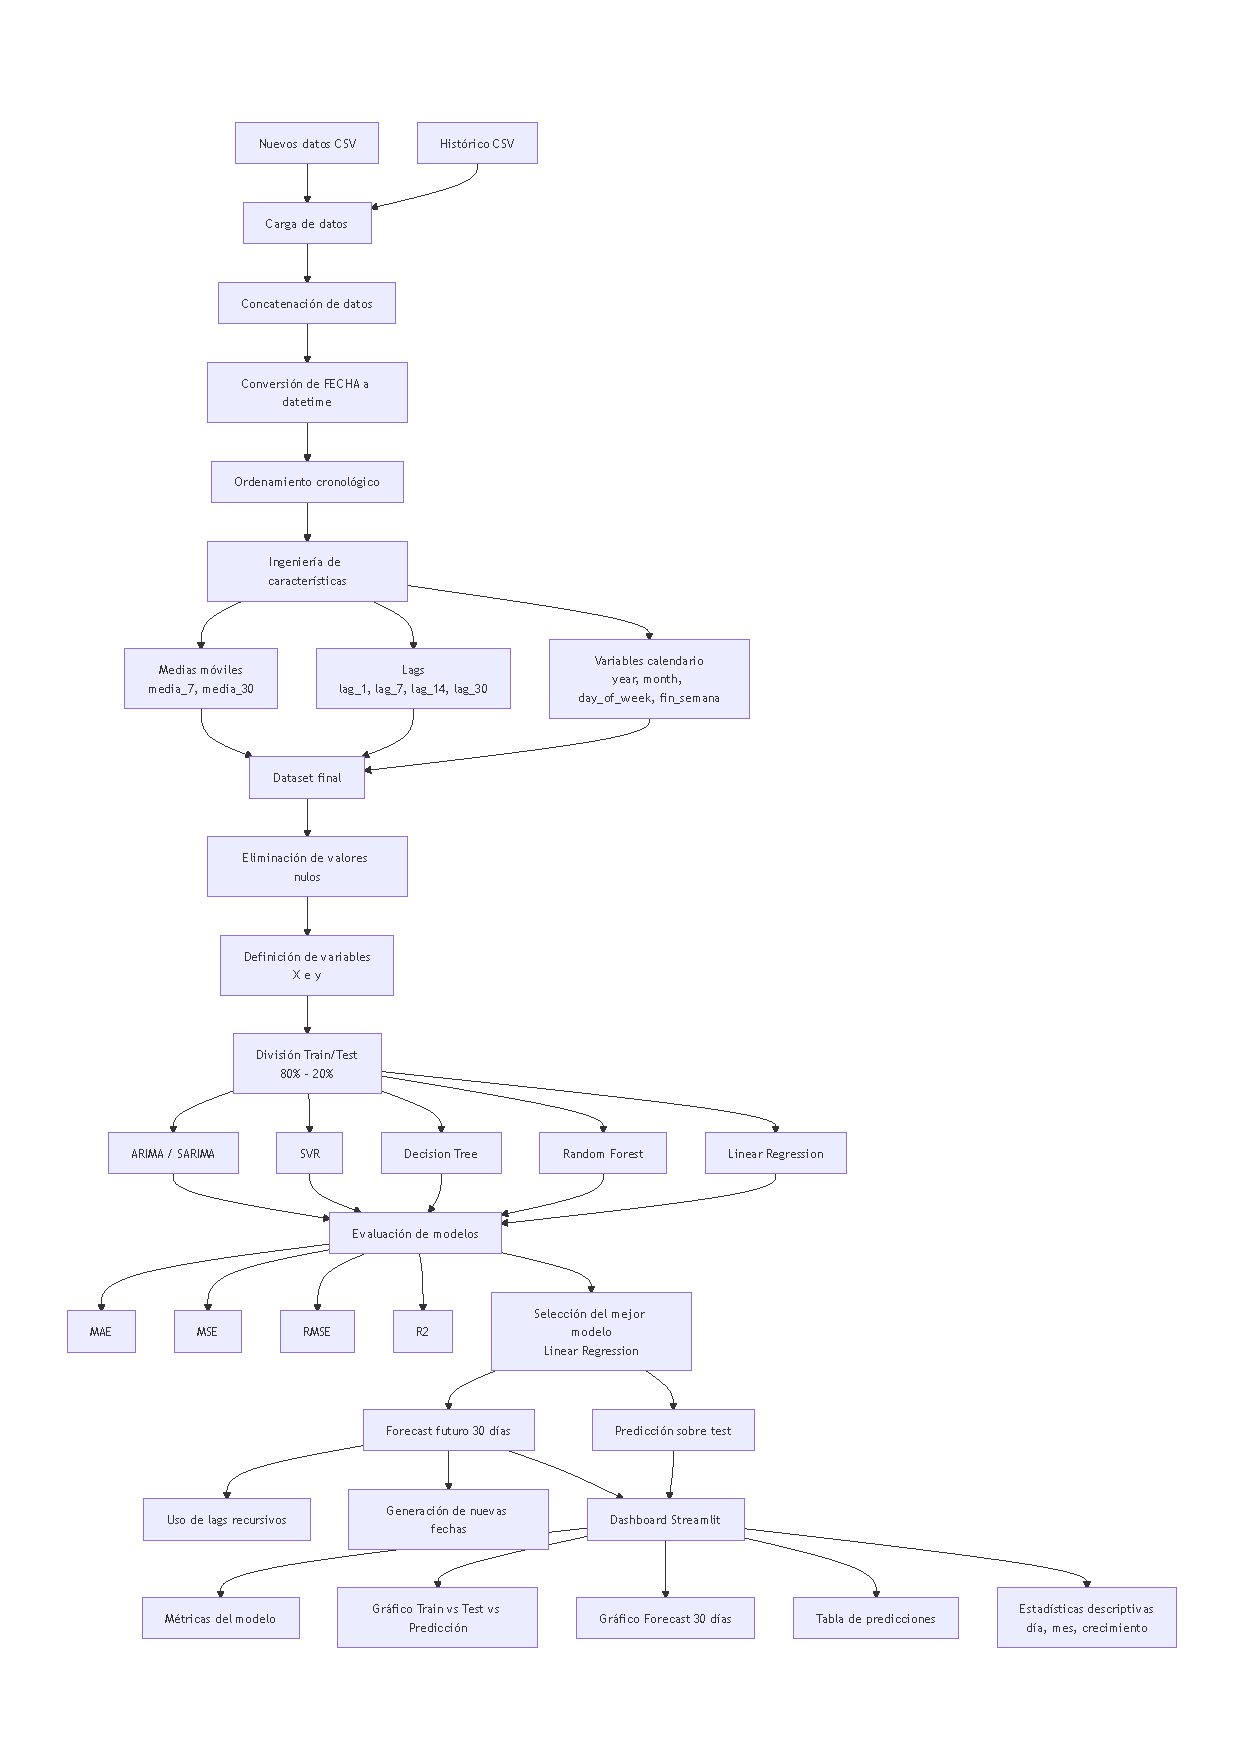
\includegraphics[width=1.05\textwidth]{anexos/arquitectura.pdf}
		\caption{Arquitectura de Software}
		\label{fig:arquitectura}
	\end{figure}


\section*{\huge Anexo III: Estados Financieros}


%%%%%%%%%%%%%%%%%%%%%%%%%%%%%%%%%%%%%%%%%%%%%%%%%%%%%%%%%%%%%%%%%%%%%%%
\subsection*{ESTADO DE GANANCIAS Y PÉRDIDAS (ENERO 2026)}

\begin{table}[H]
	\centering
	\begin{tabular}{|L{8cm}|R{4cm}|}
	\hline
	\rowcolor{yellow} LOCAL: & \cellcolor{purple!30} SAMOA \\ 
	\rowcolor{black}\textcolor{white}{PERIODO:} & \textcolor{white}{Ene-26} \\ \hline
	\rowcolor{yellow} VENTAS ORION & 273,126.10 \\ 
	\textcolor{red}{COSTO DE MERCAD VENDIDA} & 198,915.12 \\ 
	\rowcolor{gray!30} MARGEN COMERCIAL & 74,210.98 \\ 
	MERMAS & 641.27 \\ 
	PERDIDAS & 753.80 \\ 
	\rowcolor{gray!30} MARGEN BRUTO & 72,815.91 \\ 
	RRHH TIENDA & 23,886.95 \\ 
	RRHH CENTRAL & 2,183.75 \\ 
	GASTO DE COMPRA & 1,219.90 \\ 
	GASTOS DE VENTAS & 3,225.93 \\ 
	COMISION POS & 5,192.28 \\ 
	GASTO DE MKT & 152.00 \\ 
	PAGO DE SERVICIOS & 3,309.20 \\ 
	COSTOS DE LOCACION & 4,504.88 \\ 
	GASTOS FINANCIEROS & 142.21 \\ 
	\rowcolor{yellow} EBITDA & 29,283.23 \\ 
	PAGO DEUDAS & - \\ 
	INVERSIONES & 33,000.00 \\ 
	\rowcolor{yellow} EBIT & (3,716.77) \\ 
	IMPUESTOS & 2,993.40 \\ 
	\rowcolor{yellow} BENEFICIOS NETOS & (6,710.17) \\ \hline
	\end{tabular}
\caption{Fuente: Elaboración propia}
\end{table}

\vspace{1cm} % espacio entre tablas


\subsection*{FLUJO DE CAJA (ENERO 2026)}

\begin{table}[H]
	% \caption{Flujo de Caja (Tabla 1.3)}
	\centering
	\begin{tabular}{|L{8cm}|R{4cm}|}
	\hline
	\rowcolor{green!30} LOCAL: & \cellcolor{purple!30} SAMOA \\
	\rowcolor{black}\textcolor{white}{PERIODO:} & \textcolor{white}{Ene-26} \\ \hline
	SALDO INI y/o ANT & \\ 
	APALANCAMIENTO / PRESTAMOS & \\ 
	\rowcolor{green!30} VENTAS ORION & 273,126.10 \\ 
	PAGO POR MERCADERIAS & 191,255.72 \\ 
	RRHH TIENDA & 23,886.95 \\ 
	RRHH CENTRAL & 2,183.75 \\ 
	GASTO DE COMPRA & 1,219.90 \\ 
	GASTOS DE VENTAS & 3,225.93 \\ 
	COMISION POS & 5,192.28 \\ 
	GASTO DE MKT & 152.00 \\ 
	PAGO DE SERVICIOS & 3,309.20 \\ 
	COSTOS DE LOCACION & 4,504.88 \\ 
	GASTOS FINANCIEROS & 142.21 \\ 
	PAGO DE DEUDAS & - \\ 
	INVERSIONES & 33,000.00 \\ 
	IMPUESTOS & 2,993.40 \\ 
	\rowcolor{green!30} EGRESOS TOTAL & 271,066.22 \\ 
	\rowcolor{yellow} FLUJO DE CAJA & 2,059.88 \\ \hline
	\end{tabular}
\caption{Fuente: Elaboración propia}
\end{table}

Descripcion:

En enero 2026, la tienda \textbf{Samoa} tuvo ventas de \textbf{S/ 273,126.10} con un margen bruto de \textbf{S/ 72,815.91}. El \textbf{EBITDA} fue de \textbf{S/ 29,283.23}, aunque tras inversiones de \textbf{S/ 33,000} y otros gastos, el \textbf{EBIT} quedó negativo en \textbf{(S/ 3,716.77)}, resultando en una pérdida neta de \textbf{(S/ 6,710.17)}. El flujo de caja fue positivo en \textbf{S/ 2,059.88}, indicando que a pesar de los resultados contables negativos, las operaciones generaron liquidez suficiente para cubrir los compromisos inmediatos.

%%%%%%%%%%%%%%%%%%%%%%%%%%%%%%%%%%%%%%%%%%%%%%%%%%%%%%%%%%%%%%%%
\subsection*{ESTADO DE GANANCIAS Y PÉRDIDAS (FEBRERO 2026)}

%=====================
\begin{table}[H]
\centering
% \caption{Estado de Ganancias y Pérdidas (Tabla 1.4)}
\begin{tabular}{|L{8cm}|R{4cm}|}
\hline
\rowcolor{yellow} LOCAL: & \cellcolor{purple!30} SAMOA \\ 
\rowcolor{black}\textcolor{white}{PERIODO:} & \textcolor{white}{Feb-24} \\ \hline
\rowcolor{yellow} VENTAS ORION & 255,282.10 \\ 
\textcolor{red}{COSTO DE MERCAD VENDIDA} & 180,542.02 \\ 
\rowcolor{gray!30} MARGEN COMERCIAL & 74,740.08 \\ 
MERMAS & 1,693.47 \\ 
PERDIDAS & 178.30 \\ 
\rowcolor{gray!30} MARGEN BRUTO & 72,868.31 \\ 
RRHH TIENDA & 22,124.69 \\ 
RRHH CENTRAL & 2,783.75 \\ 
GASTO DE COMPRA & 1,342.50 \\ 
GASTOS DE VENTAS & 3,488.70 \\ 
COMISION POS & 4,886.10 \\ 
GASTO DE MKT & - \\ 
PAGO DE SERVICIOS & 3,724.80 \\ 
COSTOS DE LOCACION & - \\ 
GASTOS FINANCIEROS & 28.50 \\ 
\rowcolor{yellow} EBITDA & 34,546.27 \\ 
PAGO DEUDAS & - \\ 
INVERSIONES & 15,263.49 \\ 
\rowcolor{yellow} EBIT & 19,282.78 \\ 
IMPUESTOS & 2,812.20 \\ 
\rowcolor{yellow} BENEFICIOS NETOS & 16,470.58 \\ \hline
\end{tabular}
\caption{Fuente: Elaboración propia}
\end{table}

\vspace{1cm}

%=====================
\subsection*{FLUJO DE CAJA (FEBRERO 2026)}

\begin{table}[H]
\centering
% \caption{Flujo de Caja (Tabla 1.5)}
\begin{tabular}{|L{8cm}|R{4cm}|}
\hline
\rowcolor{green!30} LOCAL: & \cellcolor{purple!30} SAMOA \\
\rowcolor{black}\textcolor{white}{PERIODO:} & \textcolor{white}{Feb-24} \\ \hline
SALDO INI y/o ANT & \\ 
APALANCAMIENTO / PRESTAMOS & \\ 
\rowcolor{green!30} VENTAS ORION & 255,282.10 \\ 
PAGO POR MERCADERIAS & 184,699.99 \\ 
RRHH TIENDA & 22,124.69 \\ 
RRHH CENTRAL & 2,783.75 \\ 
GASTO DE COMPRA & 1,342.50 \\ 
GASTOS DE VENTAS & 3,488.70 \\ 
COMISION POS & 4,886.10 \\ 
GASTO DE MKT & - \\ 
PAGO DE SERVICIOS & 3,724.80 \\ 
COSTOS DE LOCACION & - \\ 
GASTOS FINANCIEROS & 28.50 \\ 
PAGO DE DEUDAS & - \\ 
INVERSIONES & 15,263.49 \\ 
IMPUESTOS & 2,812.20 \\ 
\rowcolor{green!30} EGRESOS TOTAL & 241,154.72 \\ 
\rowcolor{yellow} FLUJO DE CAJA & 14,127.38 \\ \hline
\end{tabular}
\caption{Fuente: Elaboración propia}
\end{table}

Descripcion:

En febrero 2026, las ventas descendieron a \textbf{S/ 255,282.10}, pero el margen bruto se mantuvo estable en \textbf{S/ 72,868.31}. El \textbf{EBITDA} subió a \textbf{S/ 34,546.27} y el \textbf{EBIT} fue de \textbf{S/ 19,282.78}, generando beneficios netos de \textbf{S/ 16,470.58}. El flujo de caja mejoró significativamente a \textbf{S/ 14,127.38}, reflejando un manejo más eficiente de los costos y una recuperación de liquidez, lo que indica un mejor control en la planificación de compras y mermas.

%%%%%%%%%%%%%%%%%%%%%%%%%%%%%%%%%%%%%%%%%%%%%%%%%%%%%%%%%%%%%%%%%%%%%%%%%%%%
\subsection*{ESTADO DE GANANCIAS Y PÉRDIDAS (MARZO 2026)}

\begin{table}[H]
\centering
% \caption{Estado de Ganancias y Pérdidas (Tabla 1.6)}
\begin{tabular}{|L{8cm}|R{4cm}|}
\hline
\rowcolor{yellow} LOCAL: & \cellcolor{purple!30} SAMOA \\ 
\rowcolor{black}\textcolor{white}{PERIODO:} & \textcolor{white}{Mar-24} \\ \hline
\rowcolor{yellow} VENTAS ORION & 276,817.65 \\ 
\textcolor{red}{COSTO DE MERCAD VENDIDA} & 198,176.69 \\ 
\rowcolor{gray!30} MARGEN COMERCIAL & 78,640.96 \\ 
MERMAS & - \\ 
PERDIDAS & 468.30 \\ 
\rowcolor{gray!30} MARGEN BRUTO & 78,172.66 \\ 
RRHH TIENDA & 27,444.76 \\ 
RRHH CENTRAL & 4,527.01 \\ 
GASTO DE COMPRA & 1,182.00 \\ 
GASTOS DE VENTAS & 3,945.50 \\ 
COMISION POS & 5,497.56 \\ 
GASTO DE MKT & 400.00 \\ 
PAGO DE SERVICIOS & 3,392.80 \\ 
COSTOS DE LOCACION & - \\ 
GASTOS FINANCIEROS & 28.50 \\ 
\rowcolor{yellow} EBITDA & 31,811.53 \\ 
PAGO DEUDAS & - \\ 
INVERSIONES & 14,480.33 \\ 
\rowcolor{yellow} EBIT & 17,331.20 \\ 
IMPUESTOS & 1,578.25 \\ 
\rowcolor{yellow} BENEFICIOS NETOS & 15,752.95 \\ \hline
\end{tabular}
\caption{Fuente: Elaboración propia}
\end{table}

\vspace{1cm}

%=====================
\subsection*{FLUJO DE CAJA (MARZO 2026)}
\begin{table}[H]
\centering
% \caption{Flujo de Caja (Tabla 1.7)}
\begin{tabular}{|L{8cm}|R{4cm}|}
\hline
\rowcolor{green!30} LOCAL: & \cellcolor{purple!30} SAMOA \\
\rowcolor{black}\textcolor{white}{PERIODO:} & \textcolor{white}{Mar-24} \\ \hline
SALDO INI y/o ANT & \\ 
APALANCAMIENTO / PRESTAMOS & \\ 
\rowcolor{green!30} VENTAS ORION & 276,817.65 \\ 
PAGO POR MERCADERIAS & - \\ 
RRHH TIENDA & 27,444.76 \\ 
RRHH CENTRAL & 4,527.01 \\ 
GASTO DE COMPRA & 1,182.00 \\ 
GASTOS DE VENTAS & 3,945.50 \\ 
COMISION POS & 5,497.56 \\ 
GASTO DE MKT & 400.00 \\ 
PAGO DE SERVICIOS & 3,392.80 \\ 
COSTOS DE LOCACION & - \\ 
GASTOS FINANCIEROS & 28.50 \\ 
PAGO DE DEUDAS & - \\ 
INVERSIONES & 14,480.33 \\ 
IMPUESTOS & 1,578.25 \\ 
\rowcolor{green!30} EGRESOS TOTAL & 62,476.71 \\ 
\rowcolor{yellow} FLUJO DE CAJA & 214,340.94 \\ \hline
\end{tabular}
\caption{Fuente: Elaboración propia}
\end{table}

Descripcion:
En marzo 2026, las ventas alcanzaron \textbf{S/ 276,817.65} con un margen bruto de \textbf{S/ 78,172.66}. El \textbf{EBITDA} se situó en \textbf{S/ 31,811.53} y el \textbf{EBIT} en \textbf{S/ 17,331.20}, con beneficios netos de \textbf{S/ 15,752.95}. El flujo de caja se elevó a \textbf{S/ 214,340.94}, mostrando que la empresa mantuvo un fuerte control sobre los egresos y logró una sólida generación de liquidez, consolidando la eficiencia operativa.

%%%%%%%%%%%%%%%%%%%%%%%%%%%%%%%%%%%%%%%%%%%%%%%%%%%%%%%%%%%%%%%%%%%%%%%%%%%%

%=====================
\section*{Balance General (Abril 2026)}

\begin{table}[H]
\centering
\begin{tabular}{|L{4cm}|R{2.8cm}|L{5cm}|R{3cm}|}
\hline
\rowcolor{green!20} \textbf{Activos} & & \textbf{Pasivos} & \\ \hline
Caja y bancos & S/ 98,451.00 & Pasivos corrientes & S/ 70,000.00 \\
Cuentas por cobrar & S/ 35,000.00 & Pasivos no corrientes & S/ 53,000.00 \\
Inventario optimizado & S/ 115,000.00 & Total Pasivos & S/ 123,000.00 \\
\rowcolor{orange!30} Anticipos & S/ 8,000.00 & Patrimonio & \\ 
Activos fijos netos & S/ 80,000.00 & Capital & S/ 202,840.00 \\
& & Utilidad abril & S/ 33,611.00 \\
& & Reserva (Contingencias) & -S/ 23,000.00 \\
\rowcolor{orange!30} & & Total Patrimonio & S/ 213,451.00 \\ \hline
\rowcolor{blue!20} Total Activos & S/ 336,451.00 & PASIVOS + PATRIMONIO & S/ 336,451.00 \\ \hline
\end{tabular}
\caption{Fuente: Elaboración propia}
\end{table}

\vspace{0.5cm}

%=====================
\section*{Estado de Resultados (Abril 2026)}

\begin{table}[H]
\centering
\begin{tabular}{|L{6cm}|R{4cm}|}
\hline
Ingresos & S/ 304,800.00 \\
Egreso & S/ 248,349.00 \\
\rowcolor{blue!20} Flujo Operativo & S/ 56,451.00 \\
Sistema de control & S/ 6,000.00 \\
Pago de deuda neto & S/ 2,000.00 \\
\rowcolor{blue!20} Caja neta & S/ 48,451.00 \\ \hline
\end{tabular}
\caption{Fuente: Elaboración propia}
\end{table}

\vspace{0.5cm}

%=====================
\section*{Estado de Resultados Detallado (Abril 2026)}

\begin{table}[H]
\centering
\begin{tabular}{|L{6cm}|R{4cm}|}
\hline
Ventas & S/ 289,800.00 \\
Costo de Ventas & S/ 201,200.00 \\
\rowcolor{blue!20} Margen Comercial & S/ 88,600.00 \\
Mermas & 290.00 \\
Perdidas & 150.00 \\
\rowcolor{blue!20} Margen Bruto real & 88,160.00 \\
RRHH TIENDA & 27,800.00 \\
RRHH CENTRAL & 4,800.00 \\
GASTO DE COMPRA & 1,200.00 \\
GASTOS DE VENTAS & 3,700.00 \\
COMISIÓN POS & 5,600.00 \\
GASTO DE MKT & -450.00 \\
SERVICIOS & 3,500.00 \\
LOCACIÓN & 4,500.00 \\
GASTOS FINANCIEROS & 30.00 \\
\rowcolor{blue!20} EBITDA & 37,480.00 \\
Depreciacion & 1,200.00 \\
EBIT & 36,280.00 \\
Impuestos & 1,769.00 \\
\rowcolor{blue!20} UTILIDAD NETA & 34,511.00 \\ \hline
\end{tabular}
\caption{Fuente: Elaboración propia}
\end{table}

Descripcion:
En abril 2026, tras aplicar el modelo predictivo desarrollado en la tesis para optimizar los pedidos de proveedores y reducir costos, las ventas crecieron a \textbf{S/ 289,800.00}, con un margen bruto real de \textbf{S/ 88,160.00}, evidenciando una mejora en la rentabilidad operativa. El \textbf{EBITDA} fue de \textbf{S/ 37,480.00} y el \textbf{EBIT} se ubicó en \textbf{S/ 36,280.00}, generando una utilidad neta de \textbf{S/ 34,511.00}. La caja neta disponible fue de \textbf{S/ 48,451.00} y el flujo operativo alcanzó \textbf{S/ 56,451.00}, demostrando que la aplicación del modelo permitió reducir mermas, optimizar inventarios y mejorar la liquidez, cumpliendo con el objetivo de la tesis de optimizar la toma de decisiones en los pedidos a proveedores y controlar los gastos.
En conclusión, al comparar los primeros cuatro meses del año, se observa que la implementación del modelo predictivo en abril permitió un \textbf{incremento en ventas, reducción de pérdidas y mermas}, y un \textbf{flujo de caja más saludable}, lo que confirma que el modelo está funcionando según lo previsto y aporta valor tangible a la gestión financiera y operativa de Market Donna.



	% \begin{figure}[H]
	% 	\centering
	% 	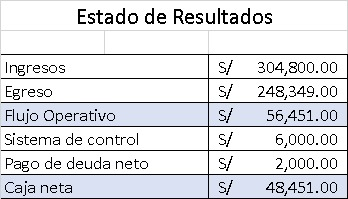
\includegraphics[width=0.8\textwidth]{anexos/er.jpeg}
	% \caption{Flujo de Efectivo}
	% 	\label{fig:flujo-efectivo}
	% \end{figure}

	% \begin{figure}[H]
	% 	\centering
	% 	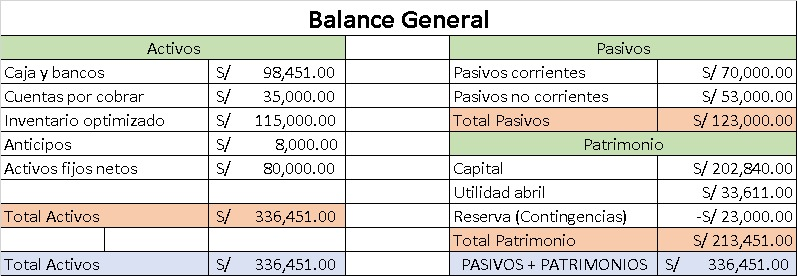
\includegraphics[width=0.8\textwidth]{anexos/bg.jpeg}
	% 	\caption{Balance General}
	% 	\label{fig:balance-general}
	% \end{figure}

	% \begin{figure}[H]
	% 	\centering
	% 	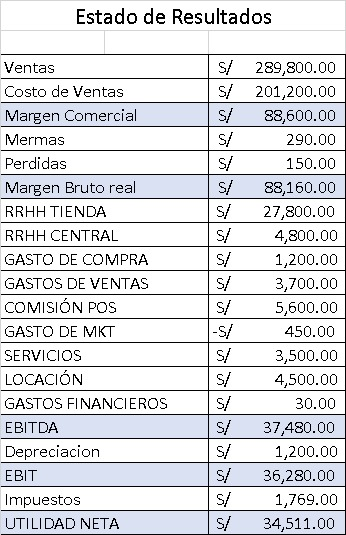
\includegraphics[width=0.8\textwidth]{anexos/fe.jpeg}
		
	% 		\caption{Estados de Resultados}
	% 	\label{fig:estados-Resultados}
	% \end{figure}

%\chapter{Anexo II: Resumen de Papers investigados}
%%\section{Conclusiones}
%
%\begin{table}[h]
%	\newcommand{\multirot}[1]{\multirow{2}{*}[-8ex]{\rotcell{\rlap{#1}}}}
%	%\scriptsize
%	\footnotesize
%	\centering
%	\begin{tabular}{|m{0.5cm}|m{0.3cm}|m{4cm}|m{2cm}|m{0.6cm}|m{1.7cm}|m{3cm}|} 
%		\hline
%		\rowcolor[rgb]{0,0.251,0.502} \multicolumn{1}{|c|}{\textcolor{white}{Tipo}} & \multicolumn{1}{c|}{\textcolor{white}{N°}} & \multicolumn{1}{c|}{\textcolor{white}{Título}}                                                                             & \multicolumn{1}{c|}{\textcolor{white}{Autor}}        & \multicolumn{1}{c|}{\textcolor{white}{Año}} & \multicolumn{1}{c|}{\textcolor{white}{País}} & \multicolumn{1}{c|}{\textcolor{white}{Fuente}}                                                        \\ 
%		\hline
%		\multirot{Problema}                                        & 1                                             & Copper price estimation using bat algorithm~                                                                               & Dehghani  Bogdanovic                                 & 2018                                        & United Kingdom                               & Resources Policy                                                                                      \\ 
%		\cline{2-7}
%		& 2                                             & Alternative techniques for forecasting mineral commodity prices                                                            & Cortez, Saydam, Coulton,  Sammut                     & 2018                                        & Netherlands                                  & International Journal of Mining Science and Technology                                                \\ 
%		\hline
%		\multirow{3}{*}[-14ex]{\rotcell{\rlap{Propuesta}}}
%		& 3                                             & Prediction of the crude oil price thanks to natural language
%		processing applied to newspapers~                           & Trastour, Genin,  Morlot                             & 2016                                        & USA                                          & Standfort University ML repository                                                                    \\ 
%		\cline{2-7}
%		& 4                                             & Stock Price Prediction Using Deep Learning~                                                                                & Tipirisetty                                          & 2018                                        & USA                                          & Master's Theses San Jose State University                                                             \\ 
%		\cline{2-7}
%		& 5                                             & Deep Learning for Stock Prediction Using Numerical and Textual
%		Information                                               & Akita, R., Yoshihara, A., Matsubara, T.,  Uehara, K. & 2016                                        & USA                                          & 2016 IEEE/ACIS 15th International Conference on Computer and
%		Information Science (ICIS)             \\ 
%		\hline
%		\multirow{4}{*}[-28ex]{\rotcell{\rlap{Técnica}}}                                          & 6                                             & Stock Prices Prediction using the Title of Newspaper Articles
%		with Korean Natural Language Processing~                   & Yun, Sim,  Seok                                      & 2019                                        & Japan                                        & 2019 International Conference on Artificial Intelligence in
%		Information and Communication (ICAIIC)  \\ 
%		\cline{2-7}
%		& 7                                             & A Method of Optimizing LDA Result Purity Based on Semantic
%		Similarity                                                    & Jingrui, Z., Qinglin, W., Yu, L.,  Yuan, L.          & 2017                                        & China                                        & 2017 32nd Youth Academic Annual Conference of Chinese
%		Association of Automation (YAC)~              \\ 
%		\cline{2-7}
%		& 8                                             & Qualitative Stock Market Predicting with Common Knowledge Based
%		Nature Language Processing: A Unified View and Procedure & Rao, D., Deng, F., Jiang, Z.,  Zhao, G.~             & 2015                                        & USA                                          & 2015 7th International Conference on Intelligent Human-Machine
%		Systems and Cybernetics              \\ 
%		\cline{2-7}
%		& 9                                             & Fuzzy Bag-of-Words Model for Document Representation                                                                       & Zhao, R.,  Mao, K.                                   & 2018                                        & USA                                          & IEEE Transactions on Fuzzy Systems (~Volume:
%		26~,~Issue: 2~, April 2018~)                           \\
%		\hline
%	\end{tabular}
%	\caption{Cuadro Resumen de Papers investigados. Fuente: Elaboración propia}
%\label{A:table}
%\end{table}




